%Chapter "Introduction"
%
\chapter{Introducción a los Elementos Finitos}
\graphicspath{{img/FEM/}}

La figura \ref{fig:chirajara} presenta el primer modo de pandeo para un pilón del puente Chirajara.
\begin{figure}[H]
    \centering
    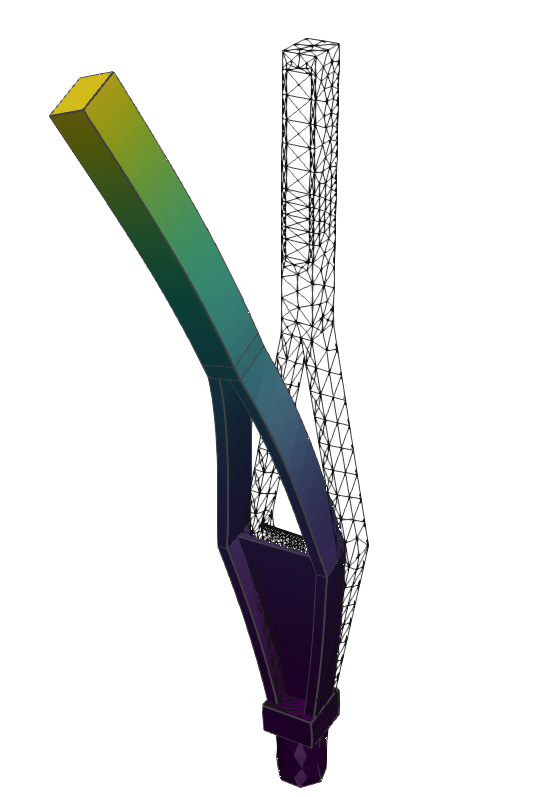
\includegraphics[width=6 cm]{pandeo_chirajara.png}
    \caption{Primer modo de pandeo para un pilón del puente Chirajara. Se 
    presenta la configuración deformada y la configuración original como 
    referencia.}
    \label{fig:chirajara}
\end{figure}

\section{Introducción}

El método de los elementos finitos es una técnica numérica para la solución de problemas de valores en la frontera propuesta inicialmente a finales de los 50 y principios de los 60  \cite{clough65, turner56}. Desde entonces, ha experimentado un fuerte desarrollo tecnológico y académico, plasmado en una gran cantidad de paquetes comerciales y de aplicaciones en diferentes áreas de ciencia e ingeniería. Paralelamente, se han escrito una gran cantidad de textos cubriendo aspectos teóricos relativos a la formulación y a la implementación del método \cite{book:bathe, book:hughes,  book:reddy, book:zienkiewicz}. En la actualidad el método de los elementos finitos puede considerarse como la herramienta de simulación numérica más poderosa y versátil para el estudio de problemas de ingeniería.

Desde el punto de vista teórico el método se basa en la solución de la forma débil del problema de valores en la frontera sobre una discretización del dominio en elementos finitos en cada uno de los cuales se expresa la solución usando interpolación a partir de valores determinados para unos cuantos puntos o nodos. La contribución de cada elemento finito del dominio es posteriormente sumada usando leyes gobernantes entre las diferentes variables del problema. En el caso mecánico la forma débil del problema de valores en la frontera corresponde al principio de los desplazamientos virtuales y el ensamblaje o consideración de todos los elementos se construye a partir de condiciones de equilibrio y compatibilidad de desplazamientos.

En ingeniería civil el método de elementos finitos es aplicable en la simulación de problemas relativos a áreas como mecánica de fluidos, análisis dinámico de estructuras, mecánica de suelos, análisis de presas, o estructuras de contención. Algunos programas comerciales, específicamente desarrollados para uso en ingeniería civil son: Plaxis\footnote{\url{http://www.plaxis.nl/plaxis2d/}}, SAP2000\footnote{\url{https://www.csiamerica.com/products/sap2000}}, OpenSees\footnote{\url{http://opensees.berkeley.edu/wiki/index.php/Main_Page}}.

A pesar del gran desarrollo del método y de su amplio uso en oficinas de 
ingeniería, especialmente en países desarrollados, este no es impartido en los 
currículos de ingeniería civil en la mayoría de universidades colombianas. En 
este capítulo se hace uso de un programa por elementos finitos desarrollado en 
Python y dirigido al análisis de sólidos elásticos en condiciones de tensión 
plana y deformación plana. El programa ha sido desarrollado principalmente con 
fines educativos en los cursos IC0285 Modelación Computacional y IC0602 
Introducción al Método de los Elementos Finitos de la Universidad EAFIT. El 
software es libre y de código abierto\footnote{La licencia es 
\href{https://opensource.org/licenses/MIT}{MIT} y puede descargarse del 
siguiente enlace: \url{https://github.com/AppliedMechanics-EAFIT/SolidsPy}.}. 
Paquetes similares, desarrollados en Python y dirigidos a uso educativo pueden 
identificarse en las herramientas SfePy \cite{sfepy}, PyFEM \cite{pyfem} and 
FEniCS \cite{fenics}.

\subsection{Aplicaciones de los elementos finitos}

El rango de aplicaciones de los elementos finitos es muy diverso, para brindar una idea de su versatilidad se presenta la siguiente lista \cite{book:first_fem}:
\begin{itemize}
	\item análisis térmico y de esfuerzos en partes industriales como circuitos integrado, dispositivos electrónicos, válvulas, tuberías, tanques, motores de autos y aviones;
	\item análisis sísmico de presas, plantas eléctricas, ciudades y edificios altos;
	\item análisis de choques de carros, trenes y aviones;
	\item análisis del flujo de contaminantes y sistemas de ventilación;
	\item análisis electromagnético de antes, transistores y aviones;
	\item análisis de procedimientos quirúrgicos como cirugías plásticas, reconstrucción de quijadas, corrección de escoliosis y muchas otras.
\end{itemize}

El uso de análisis por elementos finitos de estructuras ha reducido los ciclos de diseño considerablemente y mejorado la calidad de los productos en general. 

\section{Aspectos a tener en cuenta}


\subsection{Unidades}
La mayoría de programas de elementos finitos o simulaciones en general no cuentan con un sistema de unidades interno. Por tanto, la responsabilidad de que las unidades sean consistentes es del analista\footnote{Algunos programas sí tienen un manejo interno de las unidades. Una lista que compara algunas características está disponible en \url{www.feacompare.com}.}. Dependiendo del problema de interés, un sistema de unidades puede ser más práctico que otro\footnote{Una buena práctica es la de llevar las ecuaciones a grupos no dimensionales, ya que esto usualmente reduce la cantidad de variables independientes \cite{book:langtangen2016scaling}.}. El \cref{tab:sistema_unidades} presenta algunas cantidades y las unidades usadas para 4 sistemas consistentes de unidades.
\begin{table}[H]
\centering
\begin{tabular}{lcccc}
\hline 
\textbf{Cantidad} & \textbf{SI} & \textbf{SI (mm)} & \textbf{EEUU (ft)} & \textbf{EEUU (in)} \\ 
\hline 
Longitud & m & mm & ft & in \\ 
Fuerza & N & N & lbf & lbf \\ 
Masa & kg & tonne (10$^3$ kg) & slug & lbf s$^2$/in \\ 
Tiempo & s & s & s & s \\ 
Esfuerzo & Pa (N/m$^2$) & MPa (N/mm$^2$) & lbf/ft$^2$ & psi (lbf/in$^2$) \\ 
Energía & J & mJ (10$^{-3}$) & ft lbf & in lbf \\ 
Densidad & kg/m$^3$ & tonne/mm$^3$ & slug/ft$^3$ & lbf s$^2$/in$^4$ \\ 
\hline 
\end{tabular}
\caption{Sistemas de unidades consistentes que pueden usarse en un análisis por elementos finitos.}
\label{tab:sistema_unidades}
\end{table}

Se sugiere entonces siempre usar un sistema consistente de unidades. La presencia de las unidades se dará tanto en la geometría (las unidades de las dimensiones de la región de interés) como en los materiales.

\subsection{Materiales}
Para muchos análisis, los materiales se consideran homogéneos (no dependen de la posición) e isotrópicos (no dependen de la dirección). En algunos casos se requiere  modelar problemas en donde los materiales no son homogéneos, por ejemplo, concreto reforzado. Esta situación puede modelarse con varios subdominios con las propiedades del material de cada material constituyente.

Los siguientes cuadros presentan los valores del módulo de Young y densidad para algunos materiales comunes en ingeniería.
\begin{table}[h]
\centering
\begin{tabular}{lcccc}
\hline 
\textbf{Material} & \textbf{SI}  & \textbf{SI} & \textbf{EEUU} & \textbf{EEUU} \\
   & \textbf{(Pa)}  & \textbf{(MPa)} & \textbf{(lbf/ft$^2$)} & \textbf{(psi)} \\ 
\hline
Acero   &$200\times 10^9$ &$200\times 10^3$ &$30\times 10^6$ &$4.32\times 10^9$\\
Aluminio &$70\times 10^9$ &$70 \times 10^3$ &$10.2 \times 10^6$ &$1.46 \times 10^9$\\
Concreto & $30\times 10^9$ &$30\times 10^3$ &$648\times 10^6$ &$4.50\times 10^6$\\
\hline 
\end{tabular}
\caption{Valores de módulo de Young para algunos materiales en diferentes sistemas de unidades.}
\end{table}
\begin{table}[h]
\centering
\begin{tabular}{lcccc}
\hline 
\textbf{Material} & \textbf{SI}  & \textbf{SI} & \textbf{EEUU} & \textbf{EEUU} \\
 & \textbf{(kg/m$^3$)}  & \textbf{(kg/mm$^3$)} & \textbf{(slug/ft$^3$)} & \textbf{(lbf s$^2$/in$^4$)} \\ 
\hline
Acero   &$7800$ &$7.8 \times 10^{-6}$ &$15.2$ &$0.28$\\
Aluminio &$2700$ &$2.7 \times 10^{-6}$ &$5.24$ &$0.098$\\
Concreto & $2380$ &$2.38 \times 10^{-6}$ &$4.61$ &$0.086$\\
\hline 
\end{tabular}
\caption{Valores de densidad para algunos materiales en diferentes sistemas de unidades.}
\end{table}



\section{Geometría}

\subsection{Simplificación de la geometría}
Toda modelación que se haga de un sistema implica una idealización. Esta idealización incluye una simplificación de la geometría, es decir, despreciar algunos detalles que puedan ser de menor importancia para la estructura. Saber cuáles detalles incluir y cuáles no, no es una tarea trivial y en general dependerá de la aplicación y experiencia del analista.

Un aspecto que facilita la idealización de la geometría es la presencia de simetrías. La \cref{fig:simetrias} muestra algunos tipos de simetría que son comunes. Hay que tener en cuenta que una simetría en la geometría no necesariamente implica una simetría en la solución del problema, para ello es necesario que las condiciones de carga también sean simétricas.
\begin{figure}[H]
    \centering
    \begin{subfigure}[b]{0.49\textwidth}
    \centering
	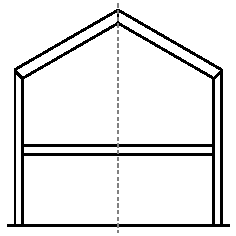
\includegraphics[height=4cm]{mirror_symmetry.pdf}
	\caption{Simetría bilateral.}
	\end{subfigure}
    \begin{subfigure}[b]{0.49\textwidth}
    \centering
	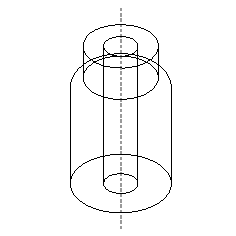
\includegraphics[height=4cm]{axial_symmetry.pdf}
	\caption{Simetría rotacional.}
	\end{subfigure}\\	
	\begin{subfigure}[b]{0.49\textwidth}
	\centering
	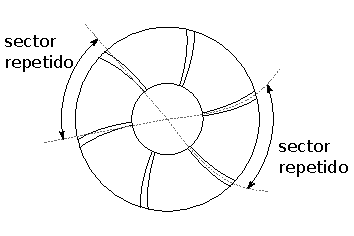
\includegraphics[height=4cm]{cyclic_symmetry.pdf}
	\caption{Simetría cíclica.}
	\end{subfigure}
    \begin{subfigure}[b]{0.49\textwidth}
    \centering
	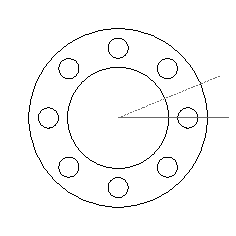
\includegraphics[height=4cm]{cyclic-mirror_symmetry.pdf}
	\caption{Simetría cíclica/bilateral.}
	\end{subfigure}\\
    \begin{subfigure}[b]{\textwidth}
    \centering
	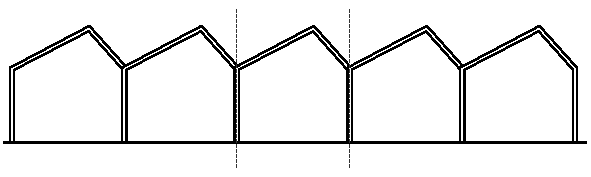
\includegraphics[height=3cm]{repetitive_symmetry.pdf}
	\caption{Simetría repetitiva.}
	\end{subfigure}\\
    \begin{subfigure}[b]{\textwidth}
    \centering
	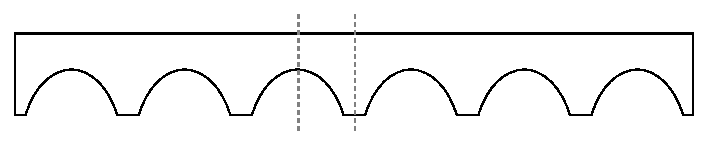
\includegraphics[height=2.5cm]{repetitive-mirror_symmetry.pdf}
	\caption{Simetría repetitiva/bilateral.}
	\end{subfigure}
    \caption{Tipos de simetrías en diferentes geometrías \cite{how_to_FEM}.}
    \label{fig:simetrias}
\end{figure}


\section{Creación y solución de un modelo de elementos finitos paso a paso}
Esta sección incluye un tutorial sobre cómo generar una geometría (específica) usando Gmsh y su posterior procesamiento para la generación de archivos de entrada para un programa de Elementos Finitos en Python\footnote{El programa de elementos finitos trabajado en clase escrito en Python que puede descargarse del sitio \url{https://github.com/AppliedMechanics-EAFIT/SolidsPy}.}.

\subsection{Modelo a resolver}
El ejemplo que se piensa resolver corresponde con la determinación de esfuerzos en un cilindro en la \emph{Prueba Brasilera}. La Prueba Brasilera  es una técnica que se usa para la medida indirecta de la resistencia de rocas. Es una técnica simple y efectiva, y por ello es comúnmente usada para medidas de rocas. En algunas ocasiones esta prueba se usa también para concreto \cite{brazilian_test}.

La siguiente figura presenta un esquema del modelo a resolver. Ya que el modelo original puede presentar desplazamientos de cuerpo rígido, se decide utilizar la simetría del problema. Entonces, el problema a resolver es un cuarto del problema original y las superficies inferior e izquierda presentan restricciones de \emph{rodillo}.
\begin{figure}[H]
    \centering
    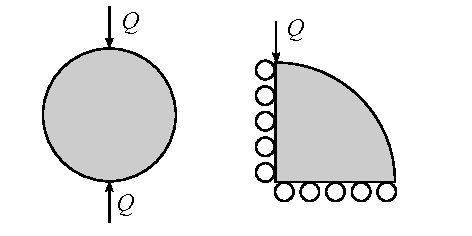
\includegraphics[height=6cm]{Prueba_brasilera.pdf}
    \caption{Esquema del modelo a resolver. A la derecha se presenta una versión de la geometría simplificada, debido a las simetrías del problema.}
\end{figure}

\subsection{Generación de la geometría y malla en Gmsh}
Como primer paso, se sugiere crear un nuevo archivo en Gmsh, como se muestra en la siguiente figura.
\begin{figure}[H]
    \centering
    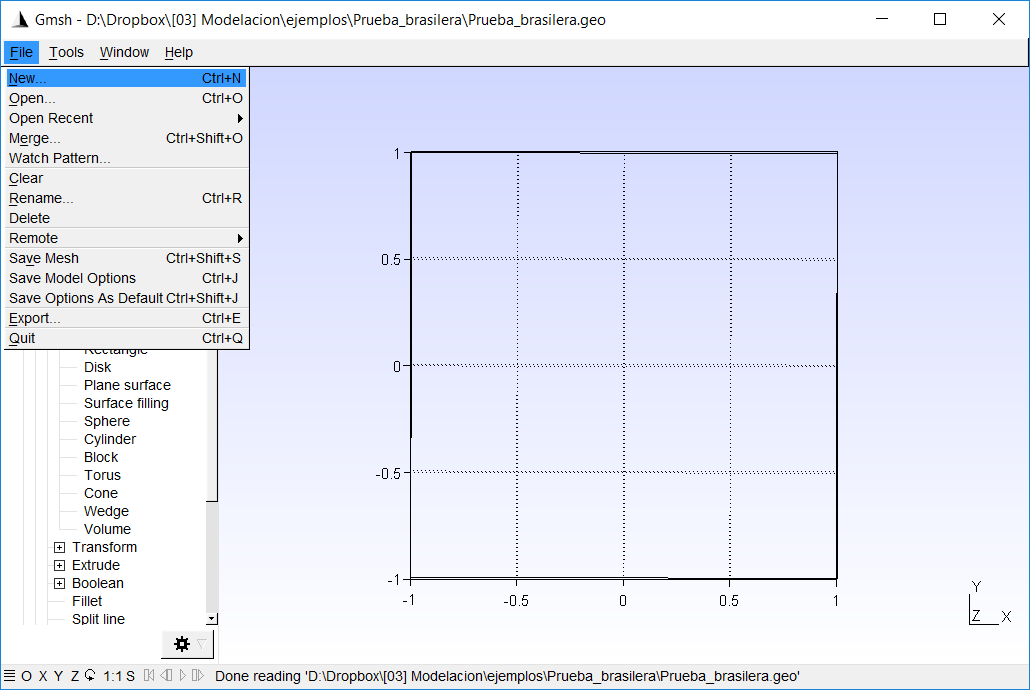
\includegraphics[height=8cm]{Nuevo_archivo.png}
    \caption{Creación de nuevo archivo en Gmsh.}
\end{figure}

Al crear un nuevo documento es posible\footnote{Si la versión es 3.0 o mayor, esta ventana emergente aparecerá} que Gmsh pregunte sobre cuál motor geométrico usar. No nos detendremos en cuáles son las diferencias y usaremos \texttt{built-in}.
\begin{figure}[H]
    \centering
    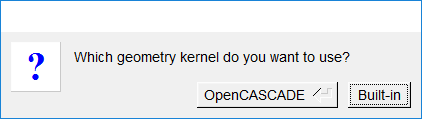
\includegraphics[height=2cm]{Motor_geometrico.png}
    \caption{Ventana emergente preguntando por el motor geométrico.}
\end{figure}

Para crear un modelo, inicialmente creamos los puntos. Para ello, vamos a la opción: \texttt{Geometry > Elementary Entities > Add > Point}, como se muestra en la siguiente figura. Luego, se añaden las coordenadas de los puntos en la ventana emergente y ``Add''. Para finalizar podemos cerrar la ventana emergente y presionar \texttt{e}.
\begin{figure}[H]
    \centering
    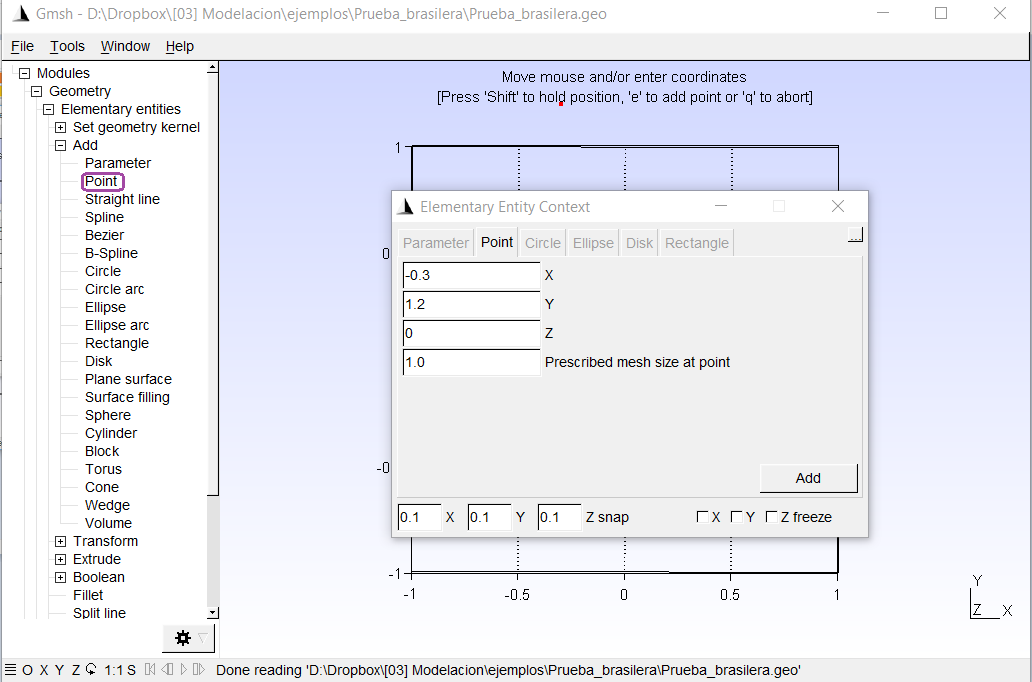
\includegraphics[height=8cm]{Agregar_puntos.png}
    \caption{Agregar puntos al modelo.}
\end{figure}

Posteriormente creamos líneas. Para ello, vamos a la opción: \texttt{Geometry > Elementary Entities > Add > Straight line}, como se muestra en la siguiente figura, y seleccionamos los puntos iniciales y finales para cada línea. Al finalizar, podemos presionar \texttt{e}.
\begin{figure}[H]
    \centering
    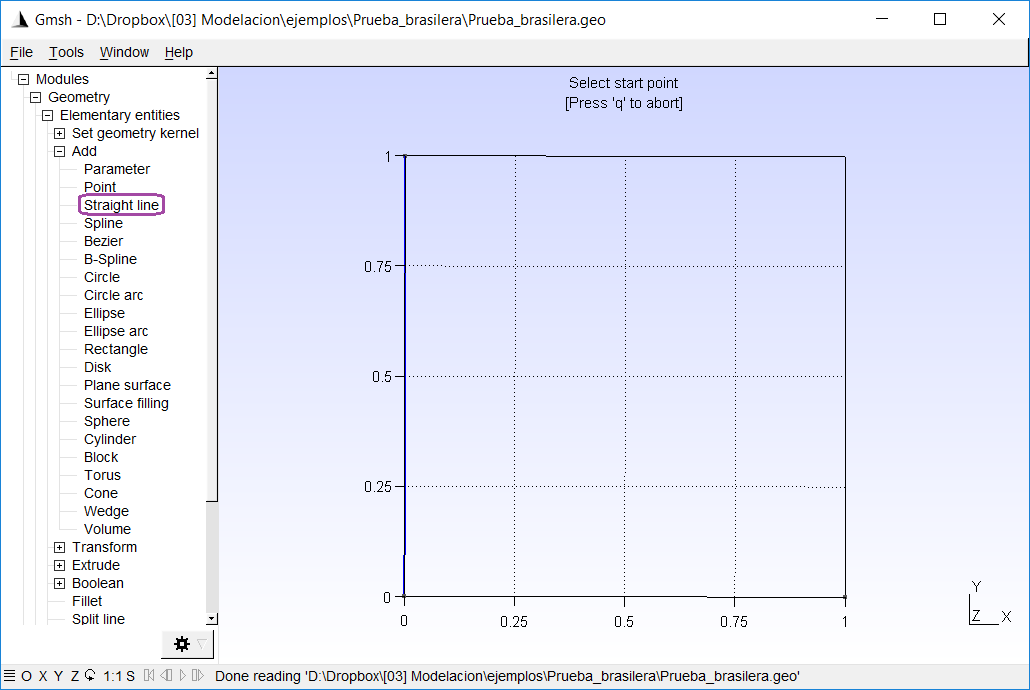
\includegraphics[height=8cm]{Agregar_lineas.png}
    \caption{Agregar líneas rectas al modelo.}
\end{figure}

También creamos los arcos de circunferencia. Para ello, vamos a la opción: \texttt{Geometry > Elementary Entities > Add > Circle Arc}, como se muestra en la siguiente figura, y seleccionamos los puntos iniciales, centrales y finales para cada arco (en ese orden). Al finalizar, podemos presionar \texttt{e}.
\begin{figure}[H]
    \centering
    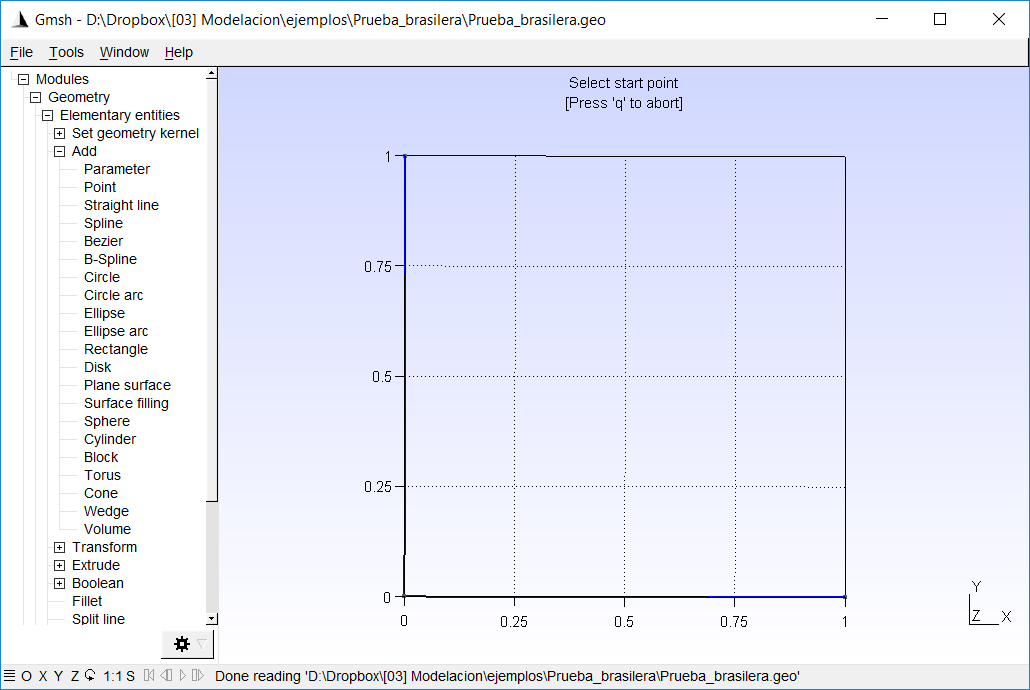
\includegraphics[height=8cm]{Agregar_arcos.png}
    \caption{Agregar arcos al modelo.}
\end{figure}

Como ya tenemos un contorno cerrado, podemos definir una superficie. Para ello, vamos a la opción: \texttt{Geometry > Elementary Entities > Add > Plane Surface}, como se muestra en la siguiente figura, y seleccionamos los contornos en orden. Al finalizar, podemos presionar \texttt{e}.
\begin{figure}[H]
    \centering
    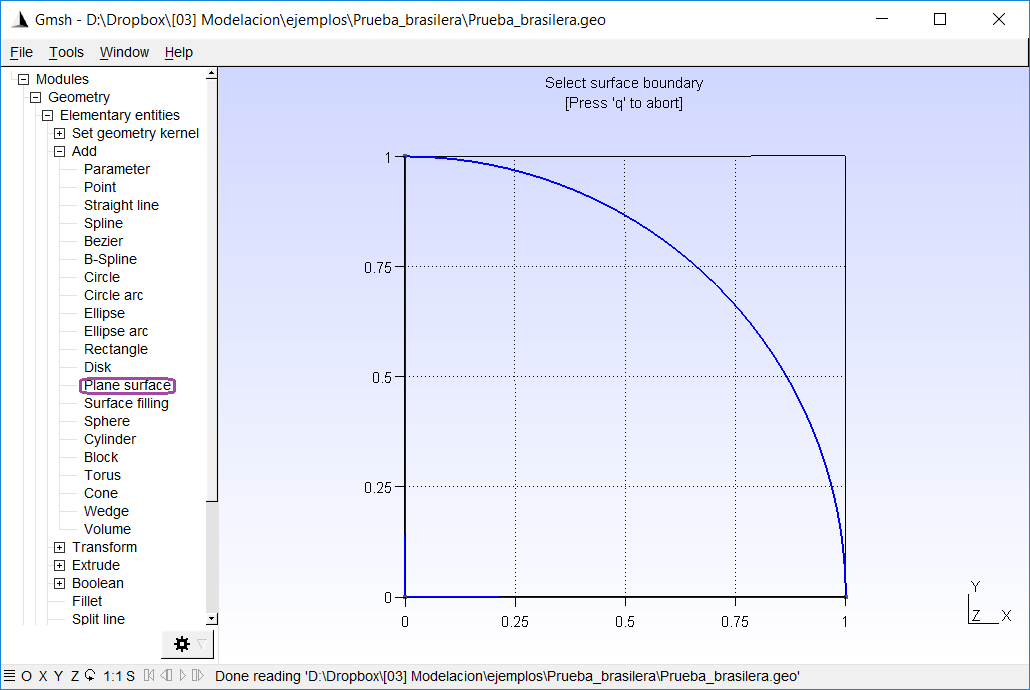
\includegraphics[height=8cm]{Agregar_superficie.png}
    \caption{Agregar superficies al modelo.}
\end{figure}

Ahora, necesitamos definir \emph{grupos físicos}. Los grupos físicos permiten asociar nombres a diferentes partes del modelo como líneas y superficies. Esto nos permitirá definir la región en la que resolveremos el modelo (y asociaremos un material), las regiones que tienen desplazamientos restringidos (condiciones de frontera) y las regiones sobre las que aplicaremos la carga. En nuestro caso tendremos 4 grupos físicos:
\begin{itemize}
    \item Región del modelo, en donde definiremos un material;
    \item Borde inferior, en donde restringiremos el desplazamiento en $y$;
    \item Borde izquierdo, en donde restringiremos el desplazamiento en $x$; y
    \item Punto superior, en donde aplicaremos la carga puntual.
\end{itemize}

Para definir los grupos físicos vamos a  \texttt{Geometry > Physical groups > Add > Plane Surface}, como muestra la siguiente figura. En este caso, podemos dejar el campo de \texttt{Name} vacío y permitir que Gmsh nombre los grupos por nosotros, los cuales serán números que luego podemos consultar en el archivo de texto.
\begin{figure}[H]
    \centering
    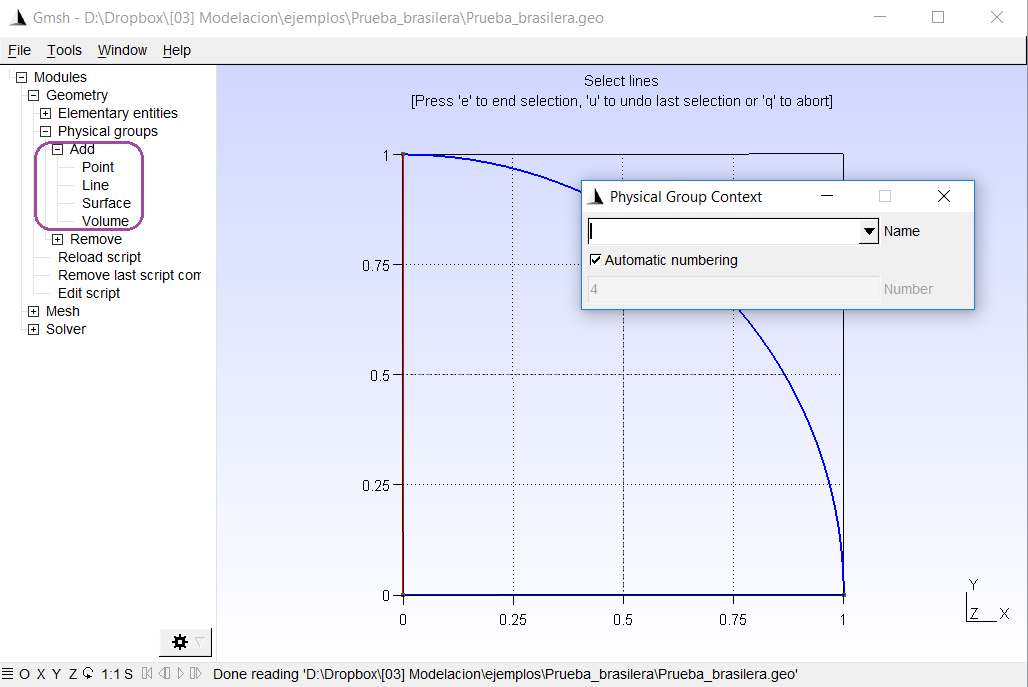
\includegraphics[height=8cm]{Agregar_linea_fisica.png}
    \caption{Agregar grupos físicos al modelo.}
\end{figure}

Luego de editar ligeramente, el archivo de texto (.geo) este luce de la siguiente manera. Agregamos un parámetro \texttt{L}, que podremos variar a nuestro antojo para cambiar el tamaño de los elementos al crear la malla.
\begin{listing}[H]
    \inputminted[mathescape,
    linenos,
    numbersep=5pt,
    gobble=0,
    frame=lines,
    framesep=2mm]{c}{src/tutorial/Prueba_brasilera.geo}
    \caption{Archivo \texttt{.geo} para el modelo descrito.}
    \label{lst:geo}
\end{listing}

Ahora, procedemos a crear la malla. Para ello,  vamos a \texttt{Mesh > 2D}.  Como vemos en la figura a continuación.
\begin{figure}[H]
    \centering
    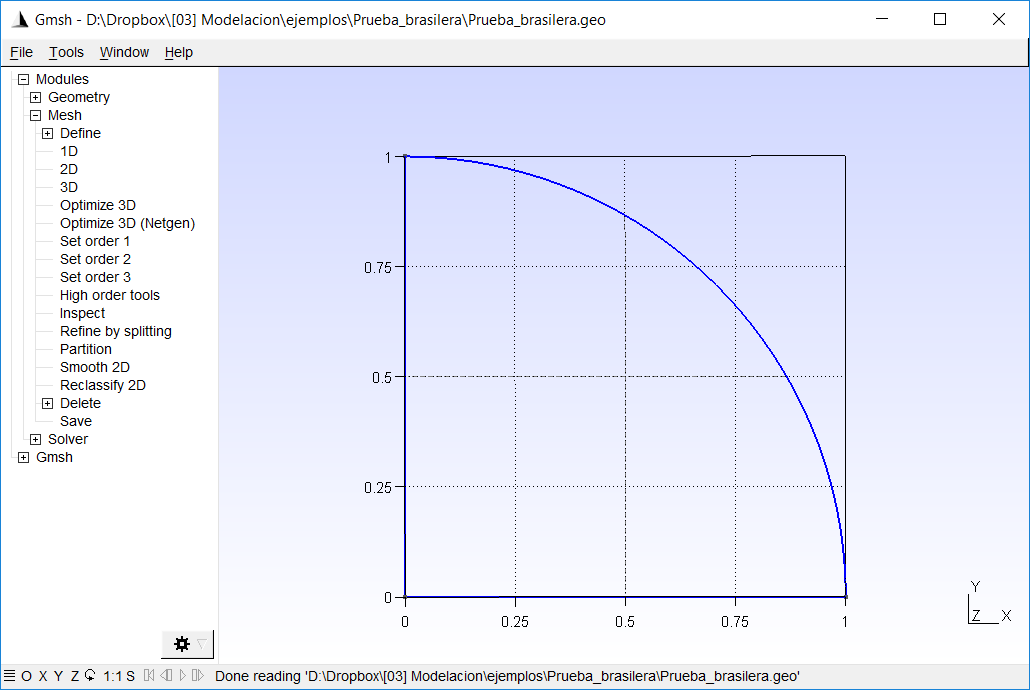
\includegraphics[height=8cm]{Mallar_2D.png}
    \caption{Crear la malla del modelo.}
\end{figure}

Adicionalmente, podemos cambiar la configuración para que muestre en colores, los elementos de la malla. Para ello, vamos a \texttt{Tools > Options > Mesh} y marcamos el cuadro que indica \texttt{Surface faces}.
\begin{figure}[H]
    \centering
    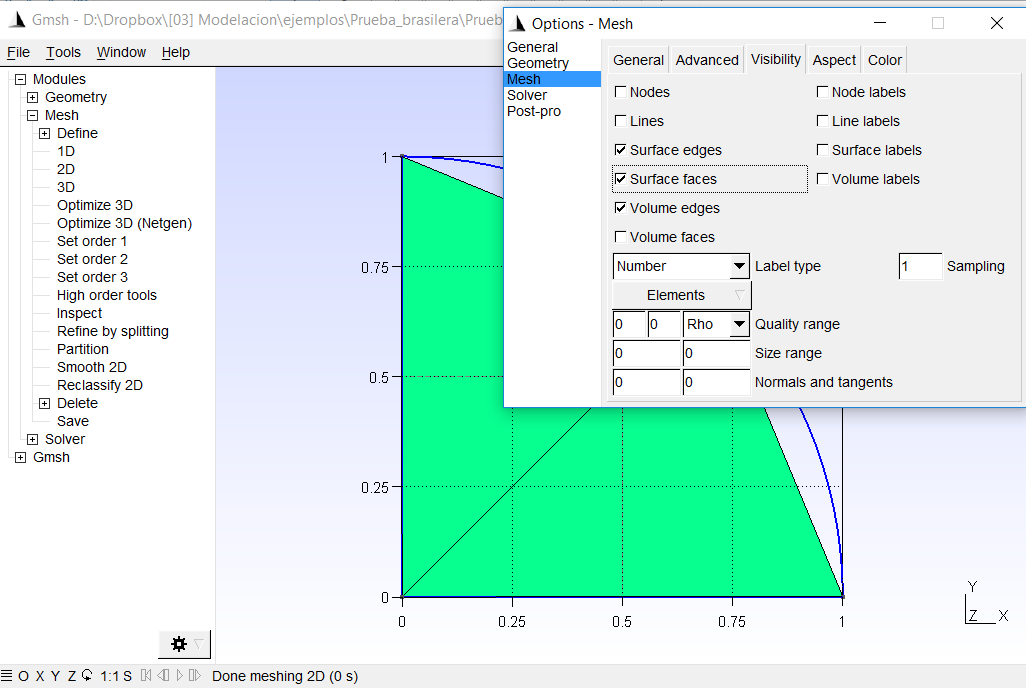
\includegraphics[height=8cm]{Ver_superficie_malla.png}
    \caption{Crear la malla del modelo.}
\end{figure}

Podemos entonces refinar la malla yendo a \texttt{Mesh > Refine by Splitting}, o midificando el parámetro \texttt{L} en el archivo de entrada (.geo). Como último paso, queremos salvar la malla. Para ello, vamos a \texttt{Mesh > Save}, o \texttt{File > Save Mesh}, como se muestra a continuación.
\begin{figure}[H]
    \centering
    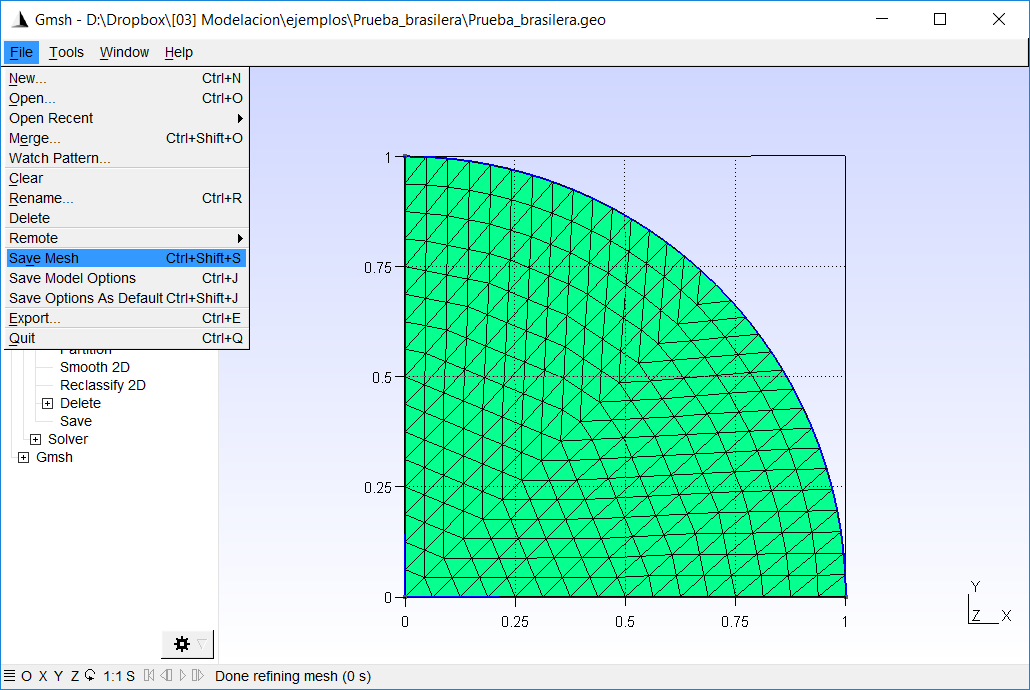
\includegraphics[height=8cm]{Grabar_malla.png}
    \caption{Guardar la malla a un archivo \texttt{.msh}.}
\end{figure}



\section{Conversión a archivos de texto}
Debemos crear archivos con la información de los nodos (\texttt{nodes.txt}), elementos (\texttt{eles.txt}), cargas (\texttt{loads.txt}) y materiales (\texttt{mater.txt}).

El siguiente código genera los archivos de entrada necesarios para correr el programa de elementos finitos en Python.
\inputminted[mathescape,
linenos,
numbersep=5pt,
gobble=0,
frame=lines,
framesep=2mm]{python}{src/tutorial/Prueba_brasilera_input.py}


Ahora, comentemos las diferentes partes del código para ver qué hace cada una.

\subsection{Encabezado y lectura de archivo \texttt{.msh}}
La primera parte carga los módulos de Python necesarios y lee el archivo de malla que en este caso se llama \texttt{Prueba\_brasilera.msh} (línea 6 y 7). Para que Python sea capaz de leer el archivo, este debe estar en el mismo directorio que el archivo de Python que lo procesará.
\begin{minted}[mathescape,
linenos,
numbersep=5pt,
gobble=0,
frame=lines,
framesep=2mm]{python}
from __future__ import division, print_function
import meshio
import numpy as np


points, cells, point_data, cell_data, field_data = \
meshio.read("Prueba_brasilera.msh")
\end{minted}

\subsection{Datos de elementos}
La siguiente sección del código crea los datos para elementos. La línea 18 crea una variable \texttt{eles} con la información de los nodos que conforman cada triángulo. La línea 19 crea un arreglo (lleno de ceros) con la cantidad de filas igual al número de elementos (\mintpy{eles.shape[0]}) y 6 columnas\footnote{Para elementos cuadriláteros se utilizarían 7 columnas, pues cada elemento está definido por 4 nodos.}. Luego asignamos un número a cada elemento, esto lo hacemos en la línea 20 con \mintpy{range(eles.shape[0])} y esto lo asignamos a la columna 0. Todos los materiales son triángulos, por eso debemos poner 3 en la columna 1. Por último, en esta sección, asignamos los nodos de cada elemento al arreglo con \mintpy{els_array} (línea 22), y esta asignación la hacemos desde la columna 3 hasta el final con \mintpy{els_array[:, 3::]}.
\begin{minted}[mathescape,
linenos,
numbersep=5pt,
gobble=0,
frame=lines,
framesep=2mm,
firstnumber=17]{python}
# Datos elementales
eles = cells["triangle"]
els_array = np.zeros([eles.shape[0], 6], dtype=int)
els_array[:, 0] = range(eles.shape[0])
els_array[:, 1] = 3
els_array[:, 3::] = eles
\end{minted}

\subsection{Datos de nodos}
En la siguiente sección creamos la información relacionada con los nodos. Para ello, en la línea 25 creamos un arreglo \mintpy{nodes_array} con 5 columnas y tantas filas como puntos tenemos en el modelo (\mintpy{point.shape[0]}). Luego, asignamos el número de elemento en la línea 26. Y, por último, asignamos la información de las coordenadas de los nodos en la línea 27 con \mintpy{nodes_array[:, 1:3] = points[:, :2]}, en donde estamos poniendo la información en las columnas 1 y 2.
\begin{minted}[mathescape,
linenos,
numbersep=5pt,
gobble=0,
frame=lines,
framesep=2mm,
firstnumber=24]{python}
# Nodos
nodes_array = np.zeros([points.shape[0], 5])
nodes_array[:, 0] = range(points.shape[0])
nodes_array[:, 1:3] = points[:, :2]
\end{minted}

\subsection{Datos de Fronteras}
En la siguiente sección encontramos la información de líneas. Para esto, leemos la información de \mintpy{cells} en la posición \mintpy{"line"}\footnote{\mintpy{cells} es un diccionario y permite almacenar información asociada a unas palabras clave, en este caso es \mintpy{"lines"}.} (línea 30). El arreglo resultante \mintpy{lines} tendrá, entonces, la información de los nodos que forman cada línea que está en la frontera del modelo. Luego, leemos la información de las líneas físicas (línea 31), y calculamos cuántas líneas pertenecen a las líneas físicas (línea 32).
\begin{minted}[mathescape,
linenos,
numbersep=5pt,
gobble=0,
frame=lines,
framesep=2mm,
firstnumber=30]{python}
# Fronteras
lines = cells["line"]
bounds = cell_data["line"]["physical"]
nbounds = len(bounds)
\end{minted}

\subsection{Datos de carga}
En la siguiente sección debemos definir la información de cargas, en este caso, las cargas las asignamos en un único punto que definimos como grupo físico. En la línea 31 leemos los nodos (en este caso, uno). Luego, creamos un arreglo que tiene tantas filas como cargas (\mintpy{nloads}) y 3 columnas. Asignamos el número del nodo al que pertenece cada carga (línea 35, las cargas en $x$ (línea 36) y las cargas en $y$ (línea 37).
\begin{minted}[mathescape,
linenos,
numbersep=5pt,
gobble=0,
frame=lines,
framesep=2mm,
firstnumber=30]{python}
# Cargas
id_cargas = cells["vertex"]
nloads = len(id_cargas)
load = -10e8 # N/m
loads_array = np.zeros((nloads, 3))
loads_array[:, 0] = id_cargas
loads_array[:, 1] = 0
loads_array[:, 2] = load
\end{minted}

\subsection{Condiciones de frontera}
Ahora, procederemos a aplicar las condiciones de frontera, es decir, las regiones del modelo que tienen restricciones en el desplazamiento. Inicialmente, identificamos cuáles líneas tienen como identificador 1 (que serían las del lado izquierdo) con

\mint{python}{id_izq = [cont for cont in range(nbounds) if bounds[cont] == 1]}

Esto crea una lista con los números (\mintpy{cont}) para los cuales se cumple la condición (\mintpy{bounds[cont] == 1}). Ahora, en la línea 46 obtenemos los nodos que pertenecen a estas líneas, sin embargo, este arreglo tiene tantas filas como líneas en el lado izquierdo y dos columnas. Primero volvemos este arreglo como un arreglo unidimensional con \mintpy{nodes_izq.flatten()}. Posteriormente, en la línea 50, asignamos el valor de -1 en la tercera columna del arreglo \mintpy{nodes_array} para los nodos que pertenezcan al lado izquierdo. De igual forma, se repite este proceso para los nodos en la frontera inferior.
\begin{minted}[mathescape,
linenos,
numbersep=5pt,
gobble=0,
frame=lines,
framesep=2mm,
firstnumber=30]{python}
# Condiciones de frontera
id_izq = [cont for cont in range(nbounds) if bounds[cont] == 1]
id_inf = [cont for cont in range(nbounds) if bounds[cont] == 2]
nodes_izq = lines[id_izq]
nodes_izq = nodes_izq.flatten()
nodes_inf = lines[id_inf]
nodes_inf = nodes_inf.flatten()
nodes_array[nodes_izq, 3] = -1
nodes_array[nodes_inf, 4] = -1
\end{minted}

\subsection{Materiales}
En la siguiente sección asignamos los materiales correspondientes a cada elemento. En este caso, sólo tenemos un material. Sin embargo, se presenta el ejemplo como si hubieran dos diferentes.  Primero, creamos un arreglo con la información de materiales en donde la primera columna representa el módulo de Young y la segunda la relación de Poisson (línea 54). Luego, leemos la información de los grupos físicos de superficies en la línea 56. Finalmente, asignamos el valor de 0 a los materiales que tengan como grupo físico 4 (ver archivo \texttt{.geo} arriba) y 1 a los otros, que en este caso serán cero (línea 57). Esta información va en la columna 2 del arreglo \mintpy{els_array}.
\begin{minted}[mathescape,
linenos,
numbersep=5pt,
gobble=0,
frame=lines,
framesep=2mm,
firstnumber=30]{python}
#  Materiales
mater_array = np.array([[186e9, 0.29],
[70e9, 0.35]])
maters = cell_data["triangle"]["physical"]
els_array[:, 2]  = [0 if mater == 4 else 1 for mater in maters]
\end{minted}

\subsection{Escritura de archivos}
La última sección usa la función \mintpy{savetxt} de \texttt{numpy} para exportar los archivos.
\begin{minted}[mathescape,
linenos,
numbersep=5pt,
gobble=0,
frame=lines,
framesep=2mm,
firstnumber=30]{python}
# Generar archivos
np.savetxt("eles.txt", els_array, fmt="%d")
np.savetxt("nodes.txt", nodes_array,
fmt=("%d", "%.4f", "%.4f", "%d", "%d"))
np.savetxt("loads.txt", loads_array, fmt=("%d", "%.6f", "%.6f"))
np.savetxt("mater.txt", mater_array, fmt="%.6f")
\end{minted}


\subsection{Solución del modelo por Elementos Finitos}
Para resolver el modelo se debe ejecutar el programa \texttt{solids\_GUI.py}\footnote{Para hacer uso de la interfaz gráfica debe estar instalado \texttt{eaygui}.}. Luego de correr este programa aparecerá una ventana emergente como se muestra a continuación. En esta ventana emergente se debe ubicar el directorio en donde están los archivos de entrada generados anteriormente. Tenga en cuenta que la apariencia de esta ventana puede variar entre sistemas operativos. También tenga en cuenta que en algunas ocasiones la ventana emergente puede quedar oculta por otras ventanas en su escritorio.
\begin{figure}[H]
    \centering
    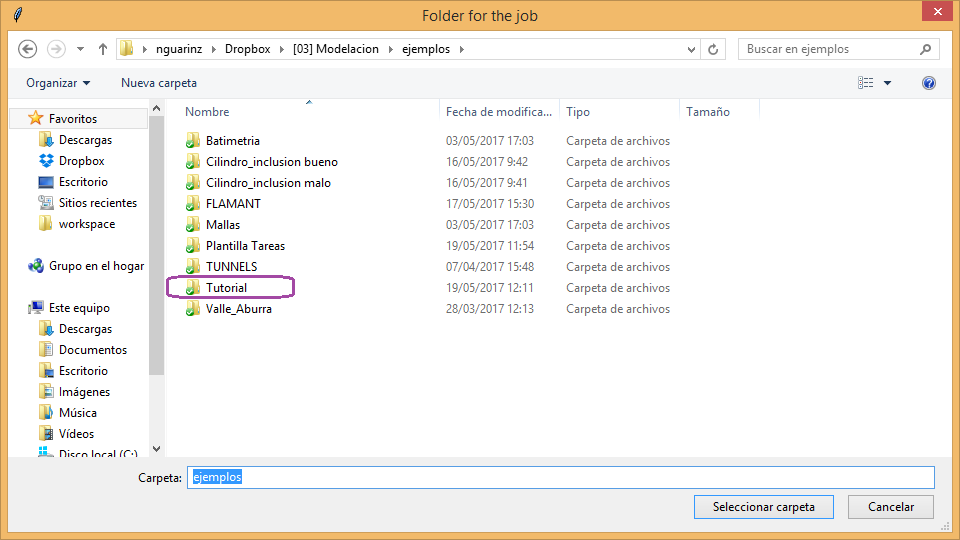
\includegraphics[height=5cm]{solids_ISO-ventana.png} 
    \caption{Ventana emergente para ubicar el directorio con los archivos de entrada.}
\end{figure}

En este punto, el programa debe resolver su modelo. Si se usan los archivos de entrada sin modificaciones el programa debe imprimir lo siguiente en la consola de Python
\begin{verbatim}
Number of nodes: 123
Number of elements: 208
Number of equations: 224
Duration for system solution: 0:00:00.086983
Duration for post processing: 0:00:00
Analysis terminated successfully!
\end{verbatim}
los tiempos que se toma en solucionar el sistema pueden cambiar un poco de un computador a otro.

Como último paso, el programa genera unos gráficos con los campos de desplazamientos, deformaciones y esfuerzos, como se muestra en la siguiente figura.
\begin{figure}[H]
    \centering
    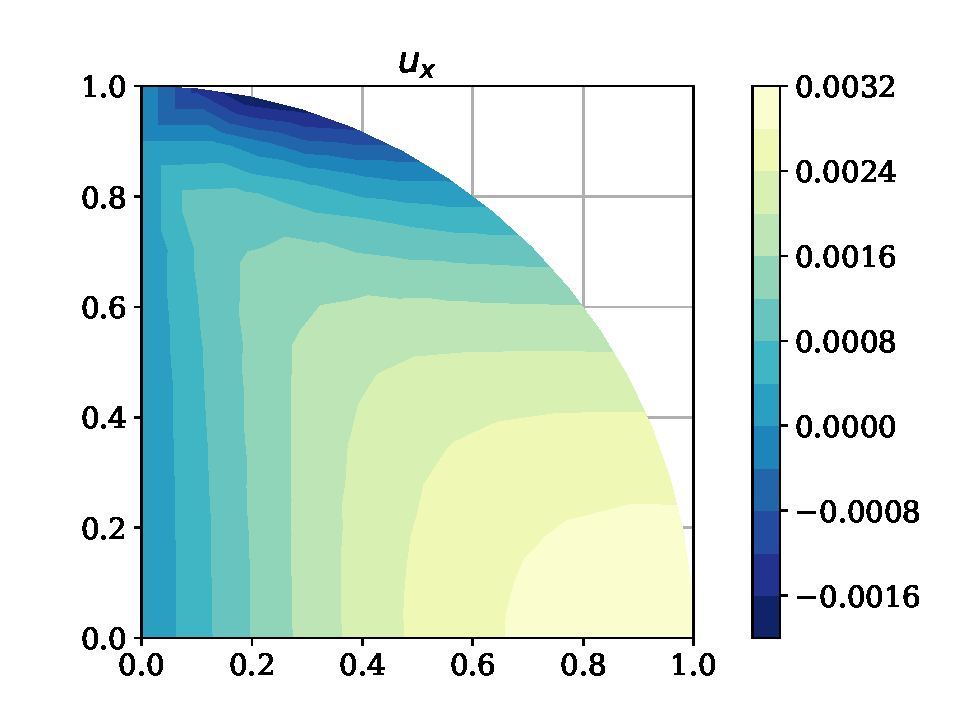
\includegraphics[height=5cm]{Prueba_brasilera_ux.pdf} 
    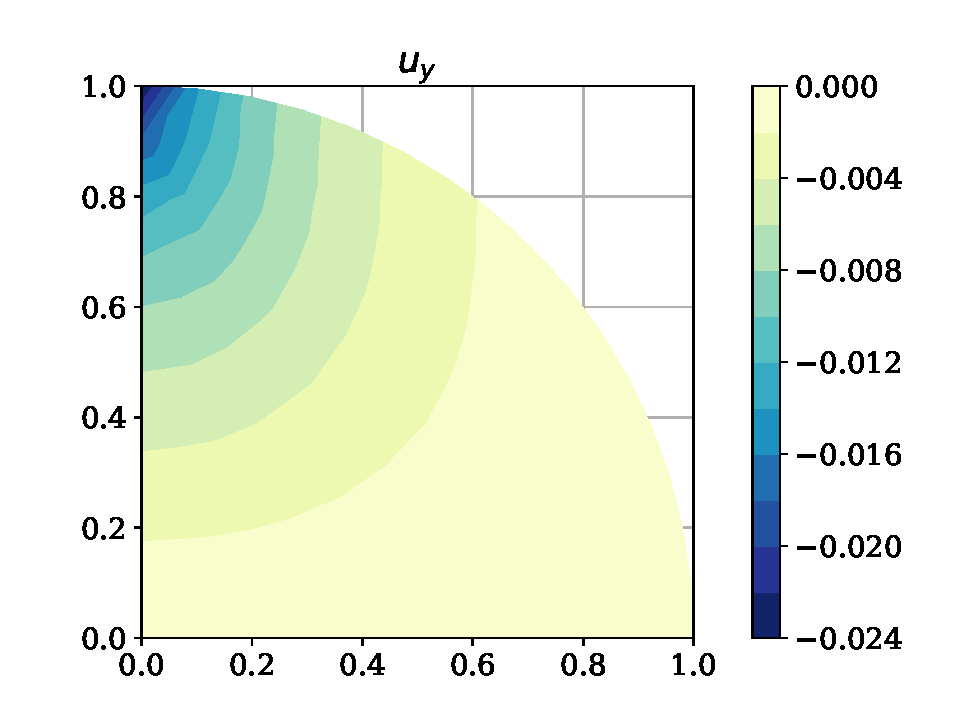
\includegraphics[height=5cm]{Prueba_brasilera_uy.pdf}
    \caption{Solución de desplazamientos para el modelo. \textbf{(Izquierda)} Desplazamientos horizontales.
    \textbf{(Derecha)} Desplazamientos verticales.}
\end{figure}


\section{Ejemplo de archivos de entrada para una malla sencilla}
Supongamos que tenemos un cuadrado de lado 1, con dos cargas en los nodos superiores y los nodos inferiores empotrados, y que está hecho de acero 1020, el cual tiene un módulo de Young $E = 186$ GPa y una relación de Poisson de $\nu = 0.29$.

Si subdividimos el cuadrado en dos triángulos, tendríamos como archivos de entrada
\begin{listing}[H]
    \begin{minted}[mathescape,
               linenos,
               numbersep=5pt,
               gobble=4,
               frame=lines,
               framesep=2mm]{python}
    0  0.0  0.0 -1 -1
    1  1.0  0.0 -1 -1
    2  1.0  1.0  0  0
    3  1.0  0.0  0  0
    \end{minted}
    \caption{Archivo \texttt{nodes.txt}.}
    \label{lst:nodes}
\end{listing}


\begin{listing}[H]
    \begin{minted}[mathescape,
               linenos,
               numbersep=5pt,
               gobble=4,
               frame=lines,
               framesep=2mm]{python}
    0  3  0  0  1  3 
    1  3  0  1  2  3
    \end{minted}
    \caption{Archivo \texttt{eles.txt}.}
    \label{lst:elements}
\end{listing}

\begin{listing}[H]
    \begin{minted}[mathescape,
               linenos,
               numbersep=5pt,
               gobble=4,
               frame=lines,
               framesep=2mm]{python}
    2  1  1
    3  1  1
    \end{minted}
    \caption{Archivo \texttt{loads.txt}.}
    \label{lst:loads}
\end{listing}

\begin{listing}[H]
    \begin{minted}[mathescape,
               linenos,
               numbersep=5pt,
               gobble=4,
               frame=lines,
               framesep=2mm]{python}
    185e9  0.29
    \end{minted}
    \caption{Archivo \texttt{mater.txt}.}
    \label{lst:mater}
\end{listing}

Si quisiéramos generar esta malla a partir de Gmsh, tendríamos como archivo \texttt{.geo}:
\begin{listing}[H]
	\inputminted[mathescape,
               linenos,
               numbersep=5pt,
               gobble=0,
               frame=lines,
               framesep=2mm]{c}{src/tutorial/Cuadrado.geo}
    \caption{Archivo \texttt{Cuadrado.geo}.}
    \label{lst:mater}
\end{listing}
